%! Author = loreb
%! Date = 31/10/2023

% Preamble
\documentclass[11pt]{article}

% Packages
\usepackage{amsmath}
\usepackage{graphicx}
\usepackage{csvsimple}
\usepackage{hyperref}
\graphicspath{{../results/plots/}}

\title{BloomFilter Speedup on setup and filter: Parallel Programming for Machine Learning}
\author{Lorenzo Baiardi, Thomas Del Moro}
\date{GG MM AAAA}

% Document
\begin{document}

    \maketitle
    \clearpage

    %\tableofcontents
    %\clearpage

    \section{Introduzione}\label{sec:introduzione}
    Il progetto consiste nella parallelizzazione di un algoritmo di Machine Learning, il BloomFilter, utilizzando il linguaggio di programmazione Python e la libreria Joblib.
    Vogliamo analizzare lo speedup ottenuto parallelizzando il BloomFilter su due principali funzioni: setup e filter.

    \section{Analisi del problema}\label{sec:analisi-del-problema}
    Il BloomFilter è una struttura dati probabilistica che permette di verificare se un elemento appartiene ad un insieme.
    In questo progetto utilizziamo il bloom filter per verificare se un email è di spam o meno, dato un insieme di email su cui effettuare il training.
    Per la inizializzazione del bloom filter è necessario fornire la probabilità di falsi positivi e la dimensione dell'insieme su cui effettuare il training.
    In base al valore della probabilità di falsi positivi e alla dimensione dell'insieme, il bloom filter calcola il numero di funzioni hash da utilizzare e la dimensione del vettore di bit che permetterà
    di memorizzare i risultati delle funzioni hash.
    La formula per il calcolo del numero di funzioni hash è la seguente:
    \begin{equation}
        k = \frac{m}{n} \ln{2}\label{eq:num_hash}
    \end{equation}
    Dove $m$ è la dimensione del vettore di bit e $n$ è la dimensione dell'insieme.
    La formula per il calcolo della dimensione del vettore di bit è la seguente:
    \begin{equation}
        m = -\frac{n \ln{p}}{(\ln{2})^2}\label{eq:dim_bit}
    \end{equation}
    Una volta passato il dataset di training al bloom filter, questo calcola per ogni email le $k$ funzioni hash e setta a 1 i bit corrispondenti alle posizioni calcolate.
    Per verificare se un email è di spam o meno, il bloom filter calcola le $k$ funzioni hash e verifica se i bit corrispondenti alle posizioni calcolate sono settati a 1.

    \section{Parallelizzazione}\label{sec:parallelizazzione}
    \subsection{Joblib}\label{subsec:joblib}
    Joblib è una libreria Python che permette di parallelizzare funzioni e cicli for.
    La funzione Parallel prende in input il numero di processori da utilizzare e la funzione da parallelizzare.
    In questo elaborato abbiamo utilizzato la funzione Parallel per parallelizzare la funzione setup e la funzione filter del bloom filter.
    Abbiamo poi successivamente elaborato quanto tempo impiegano le funzioni setup e filter a seconda del numero di processori utilizzati rispetto al tempo impiegato nella sua versione sequenziale.
    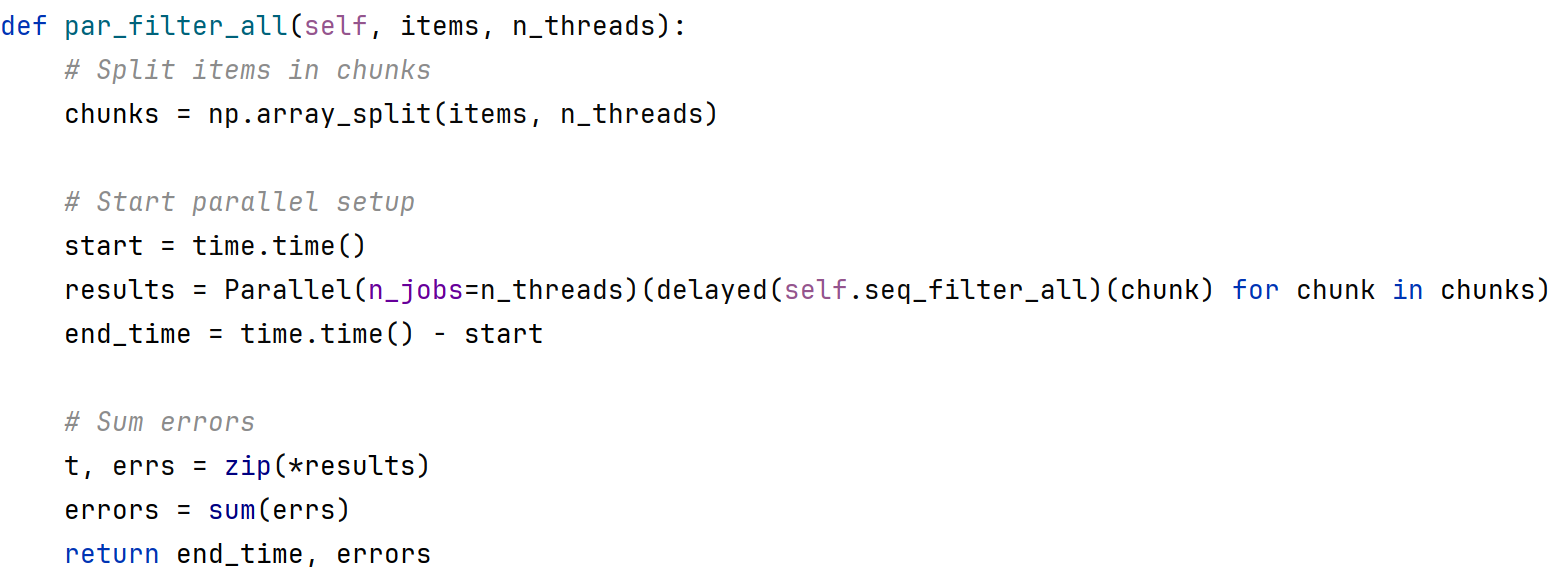
\includegraphics[width=\textwidth]{../documentation/img/pycode/pycode (1)}
    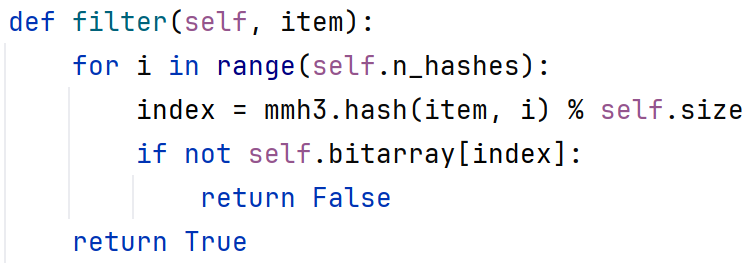
\includegraphics[width=\textwidth]{../documentation/img/pycode/pycode (2)}
    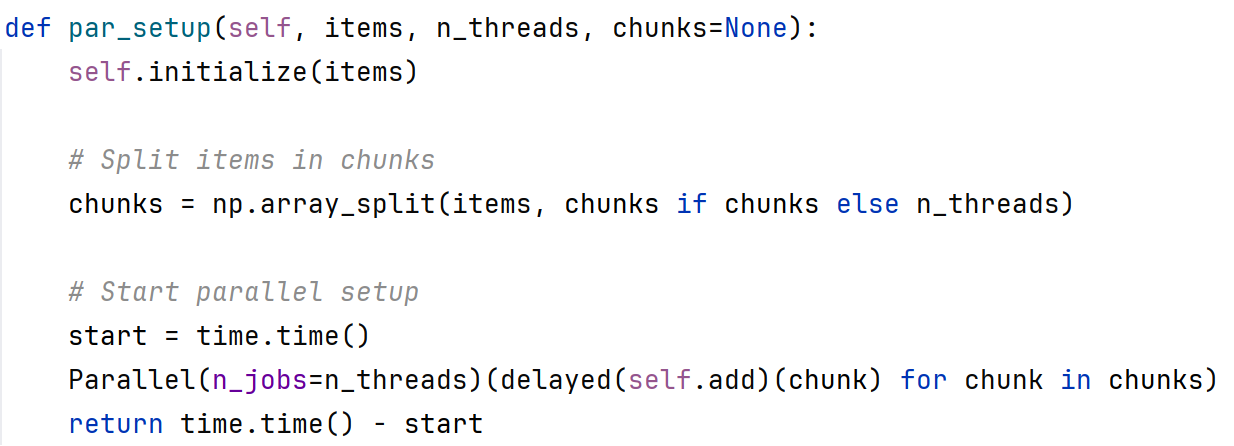
\includegraphics[width=\textwidth]{../documentation/img/pycode/pycode (3)}
    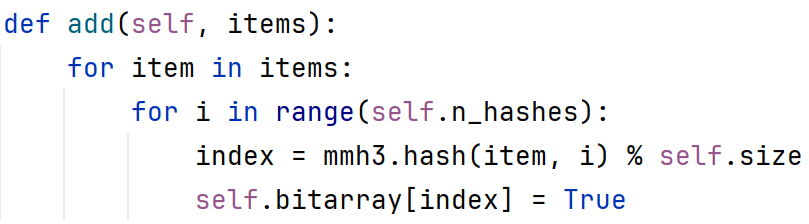
\includegraphics[width=\textwidth]{../documentation/img/pycode/pycode (4)}

    \subsection{Omp}\label{subsec:omp}
    Omp è una libreria C che permette di parallelizzare funzioni e cicli for.
    La funzione omp parallel prende in input il numero di processori da utilizzare e la funzione da parallelizzare.
    In questo elaborato abbiamo utilizzato la funzione omp parallel per parallelizzare la funzione setup e la funzione filter del bloom filter.
    Abbiamo poi successivamente elaborato quanto tempo impiegano le funzioni setup e filter a seconda del numero di processori utilizzati rispetto al tempo impiegato nella sua versione sequenziale.
    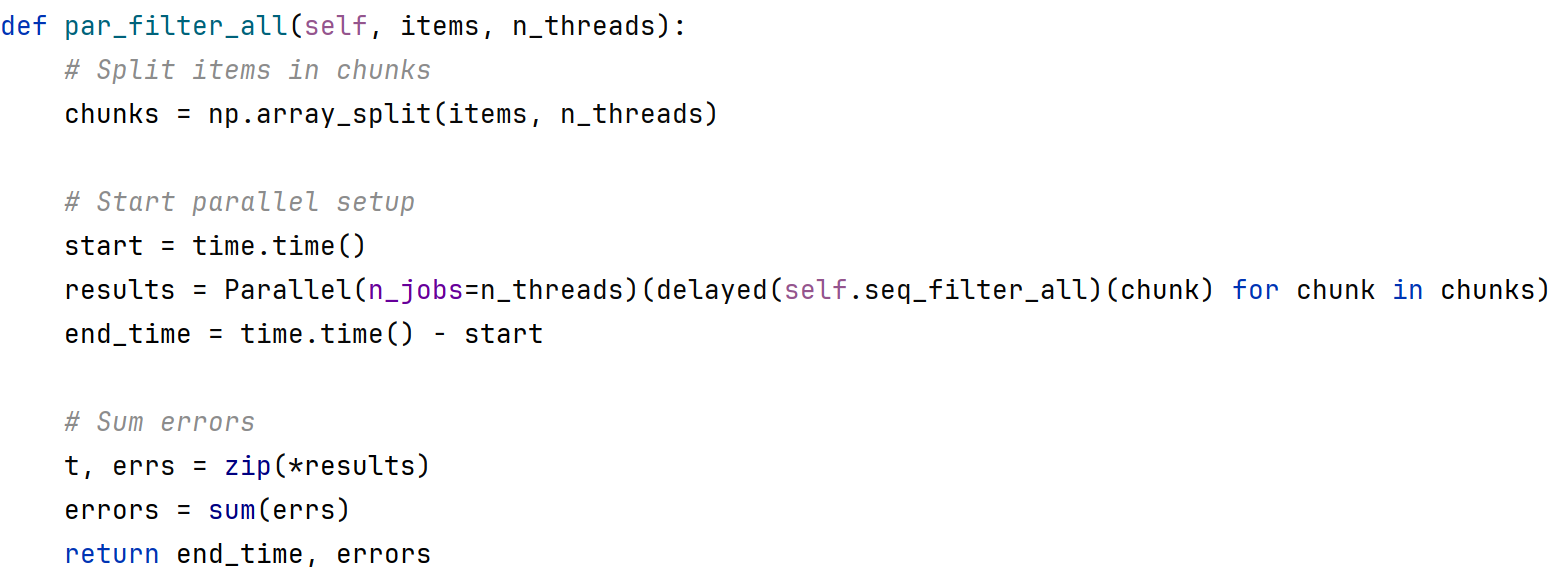
\includegraphics[width=\textwidth]{../documentation/img/pycode/pycode (1)}

    \section{Tests}\label{sec:tests}
    I test sono stati effettuati su un dataset fino a 100000 email, con una probabilità di falsi positivi pari a 0.01.
    Mentre la probabilità di falsi positivi è rimasta costante, la dimensione dell'insieme è stata variata da 1000 a 100000 email per verificare come varia lo speedup al variare della dimensione dell'insieme.
    Ci aspettiamo che per i primi test, con un numero di email minore, lo speedup sia inferiore rispetto alla versione sequenziale dovuto alla creazione dell'ambiente che permette la parallelizzazione dei processi.
    Con l'aumento invece delle email, ci aspettiamo che lo speedup aumenti fino ad un certo punto.

    \begin{figure}
        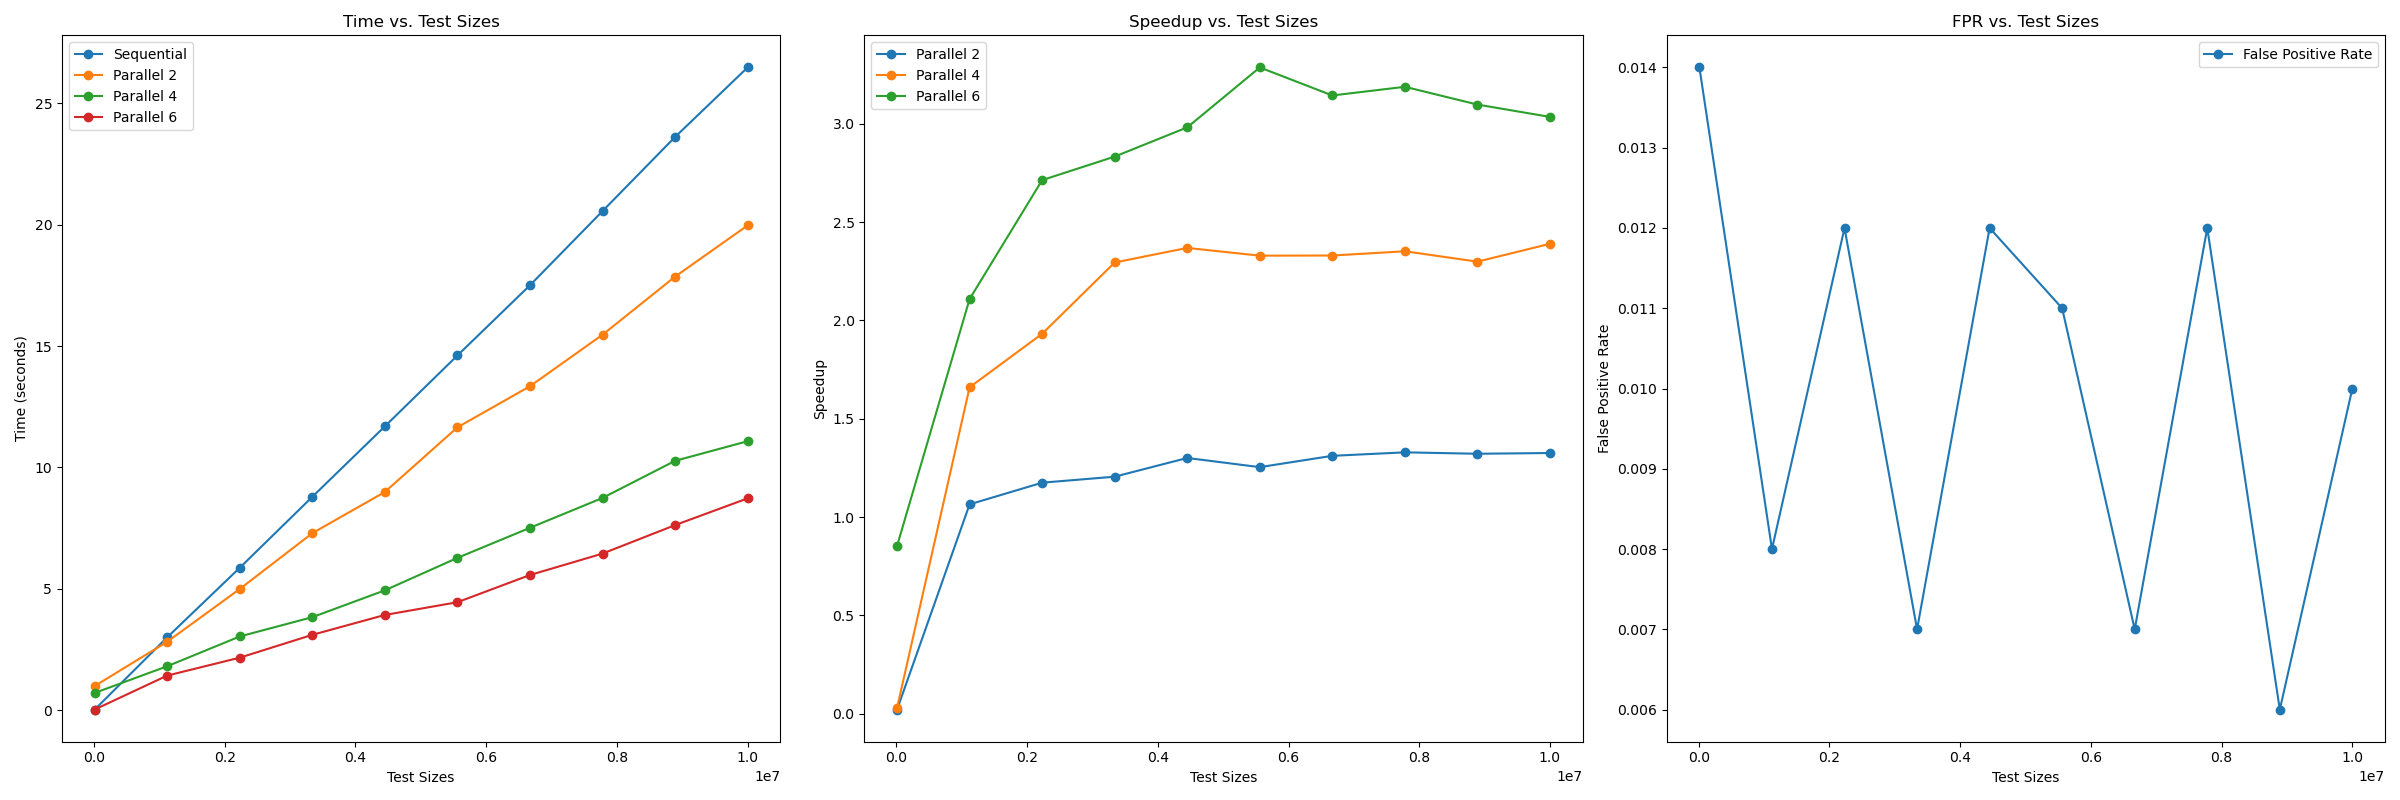
\includegraphics[width=\textwidth]{plot_setup}
        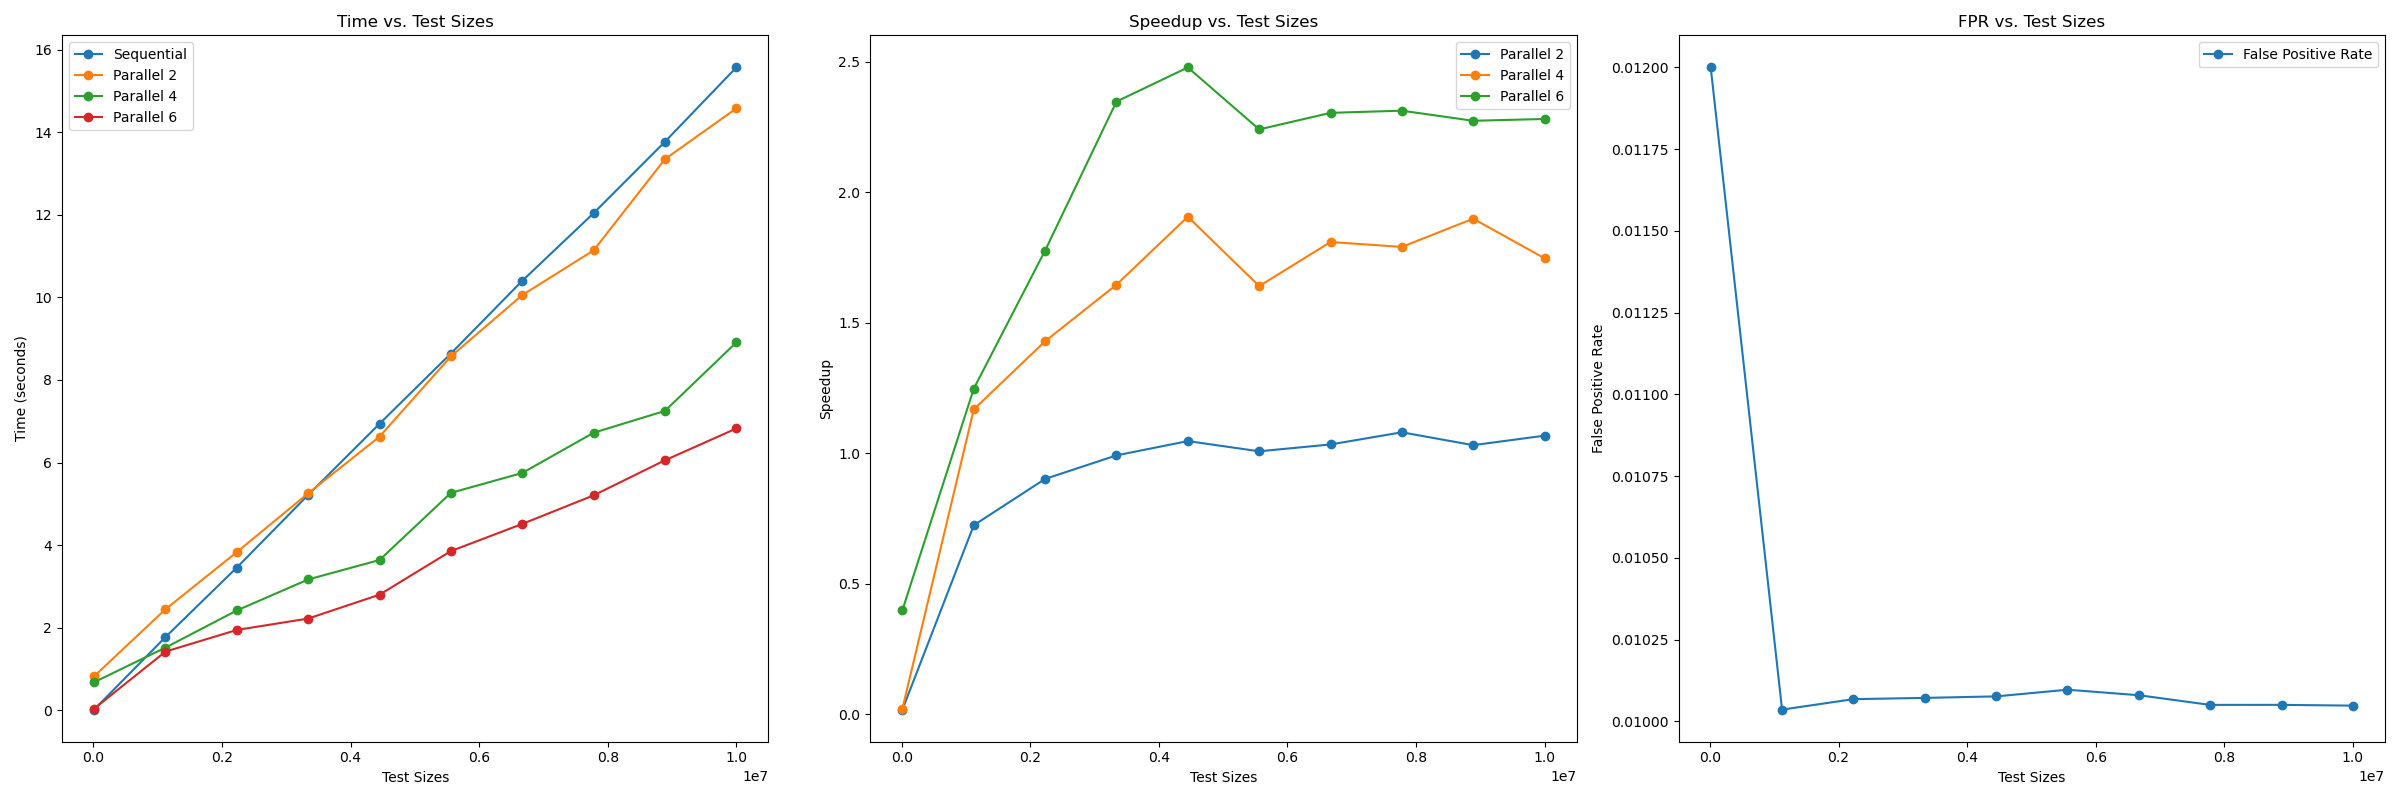
\includegraphics[width=\textwidth]{plot_filter}
        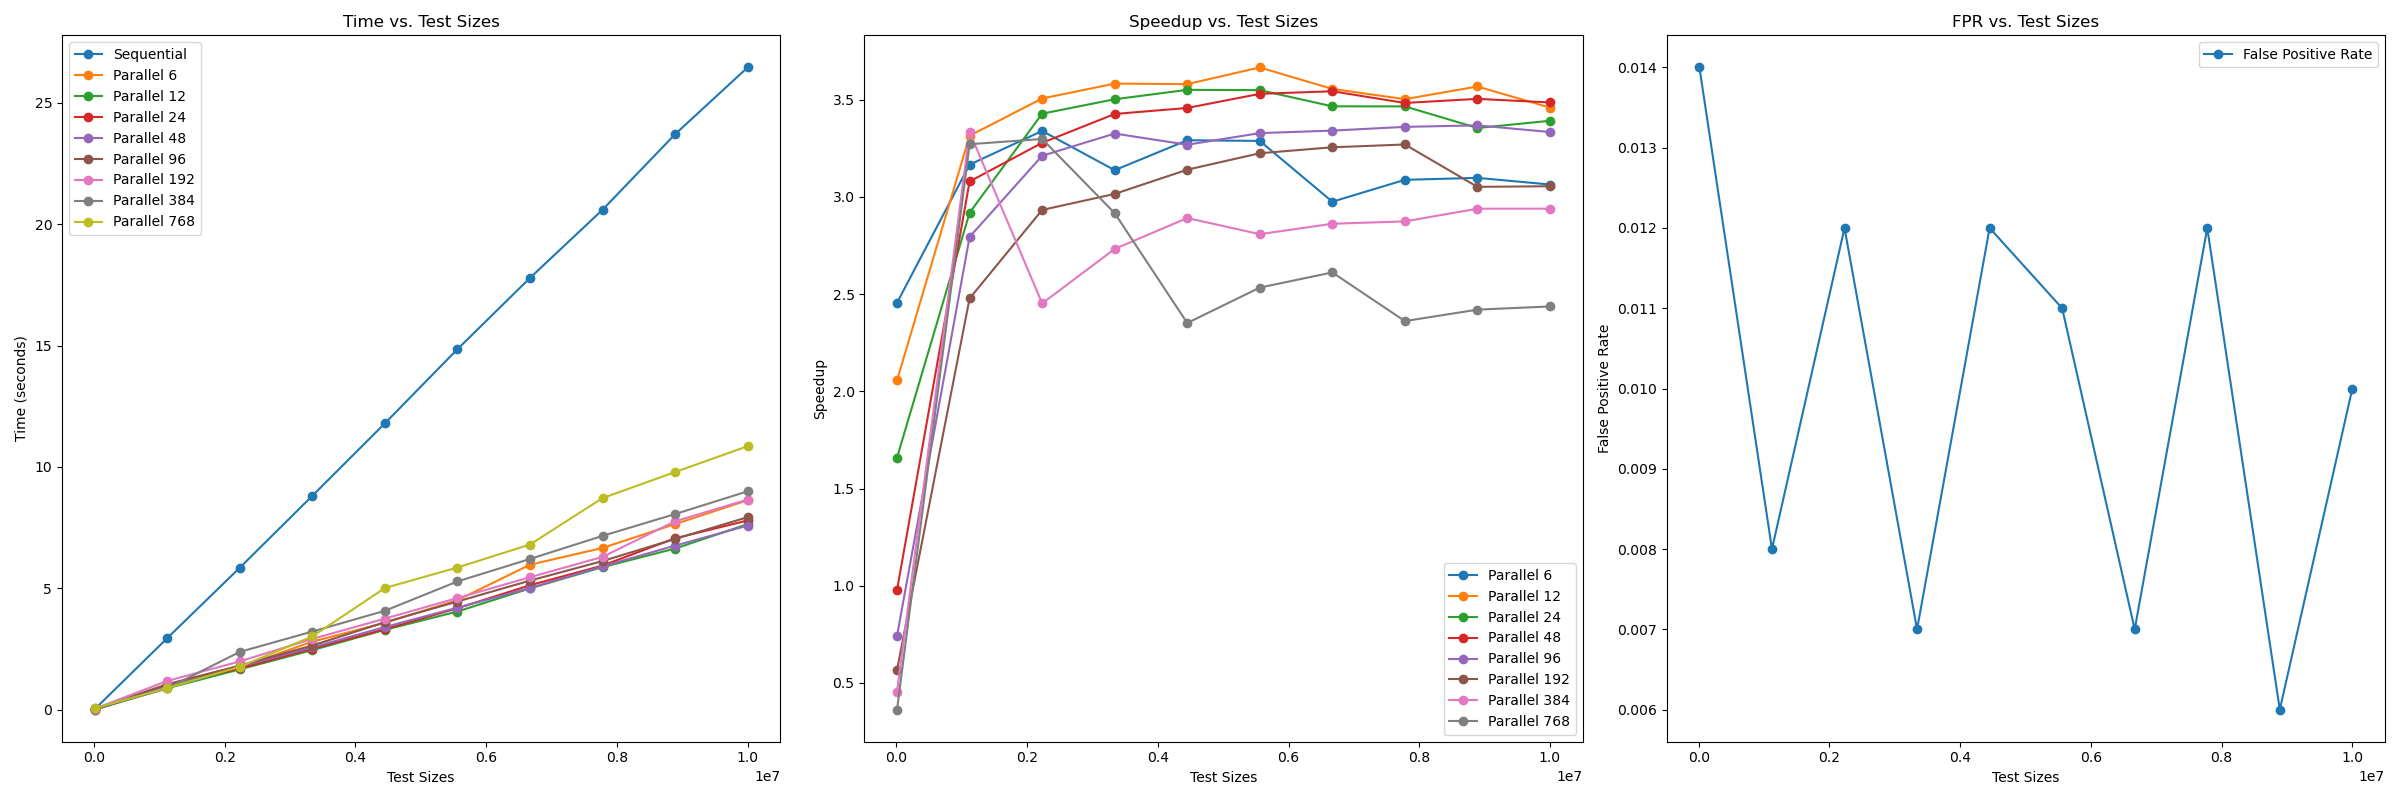
\includegraphics[width=\textwidth]{plot_chunks}
        \caption{Risultati dei test Joblib}\label{fig:joblib-result}
    \end{figure}

    \begin{figure}
        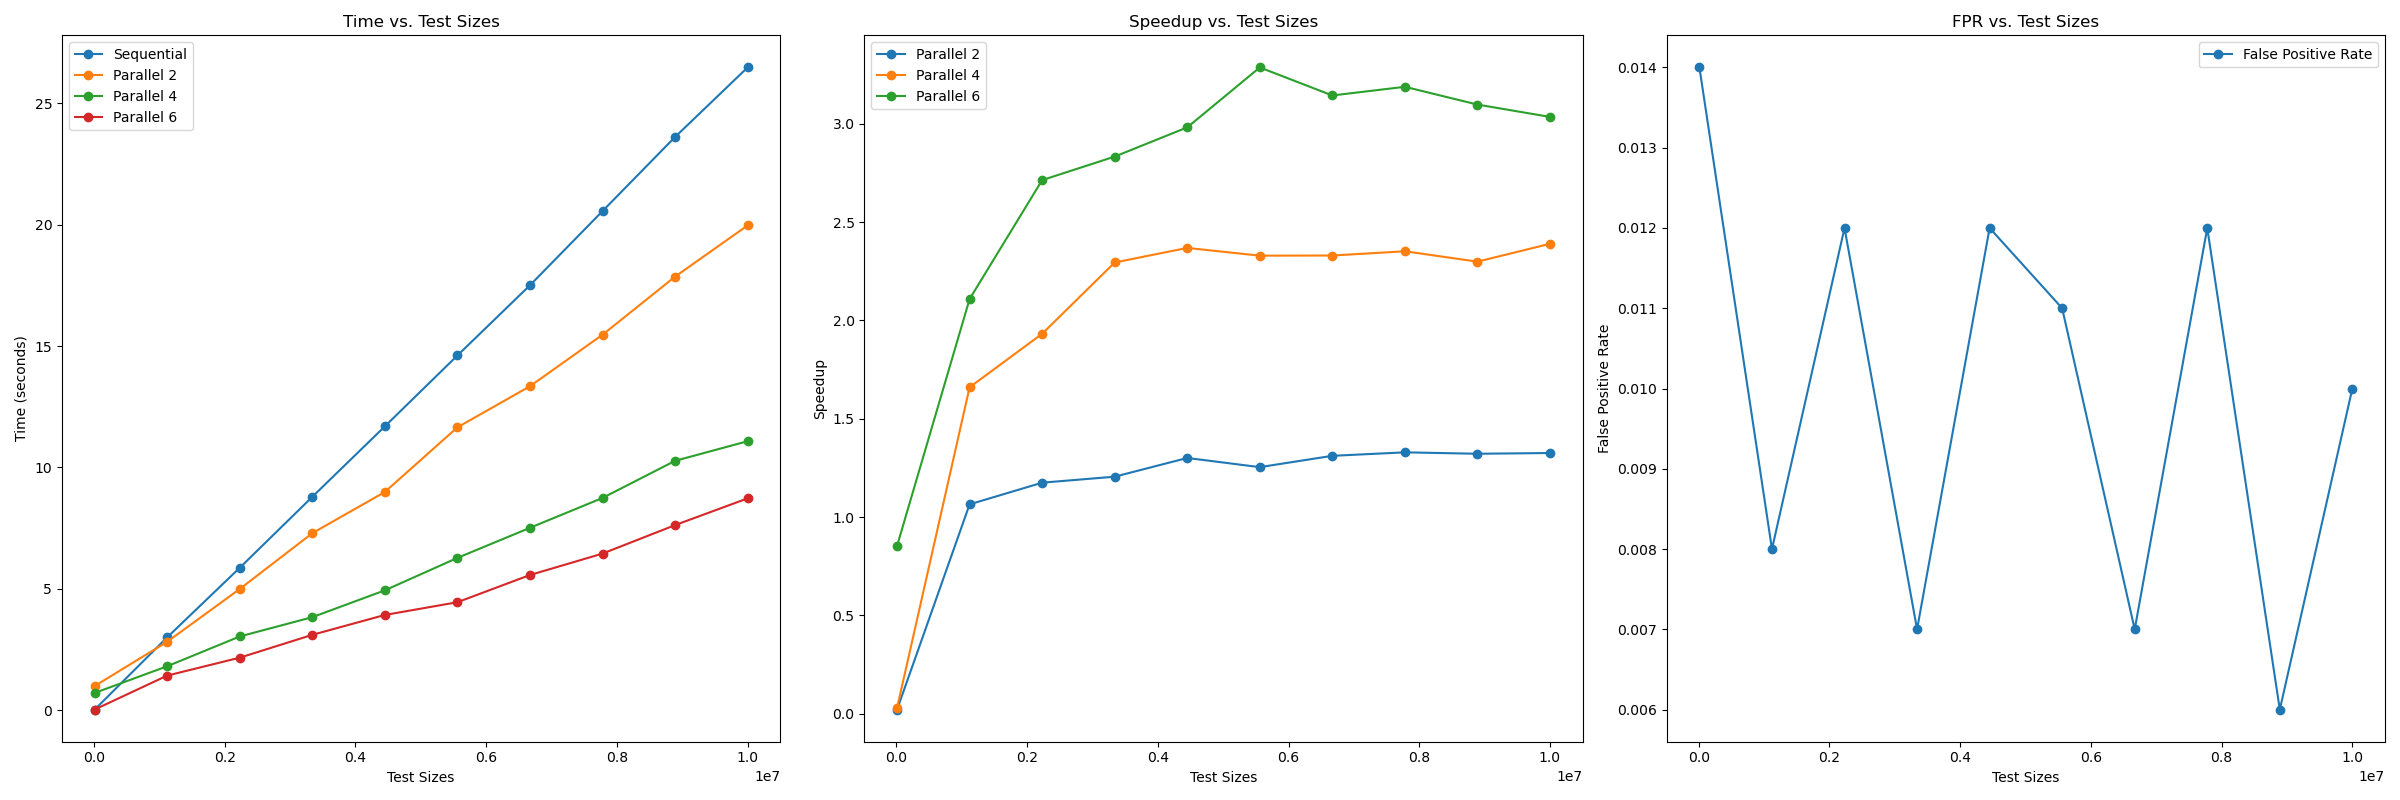
\includegraphics[width=\textwidth]{plot_setup}
        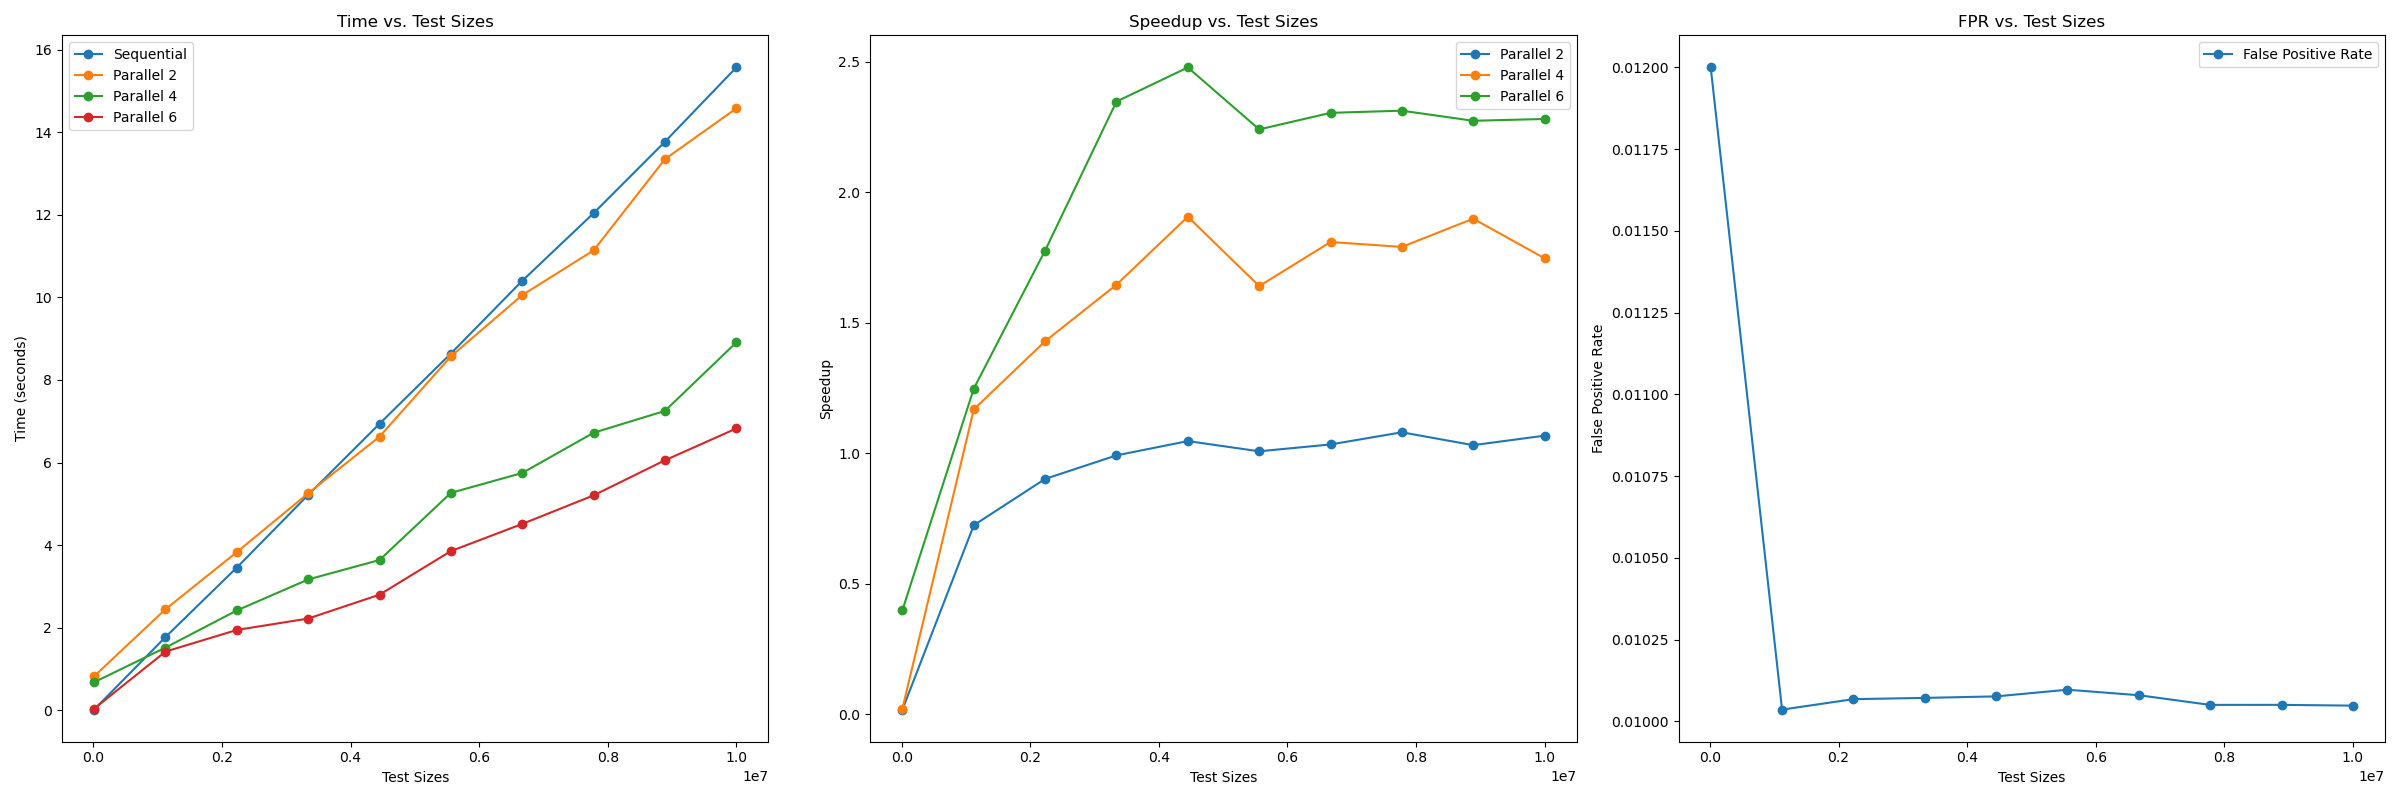
\includegraphics[width=\textwidth]{plot_filter}
        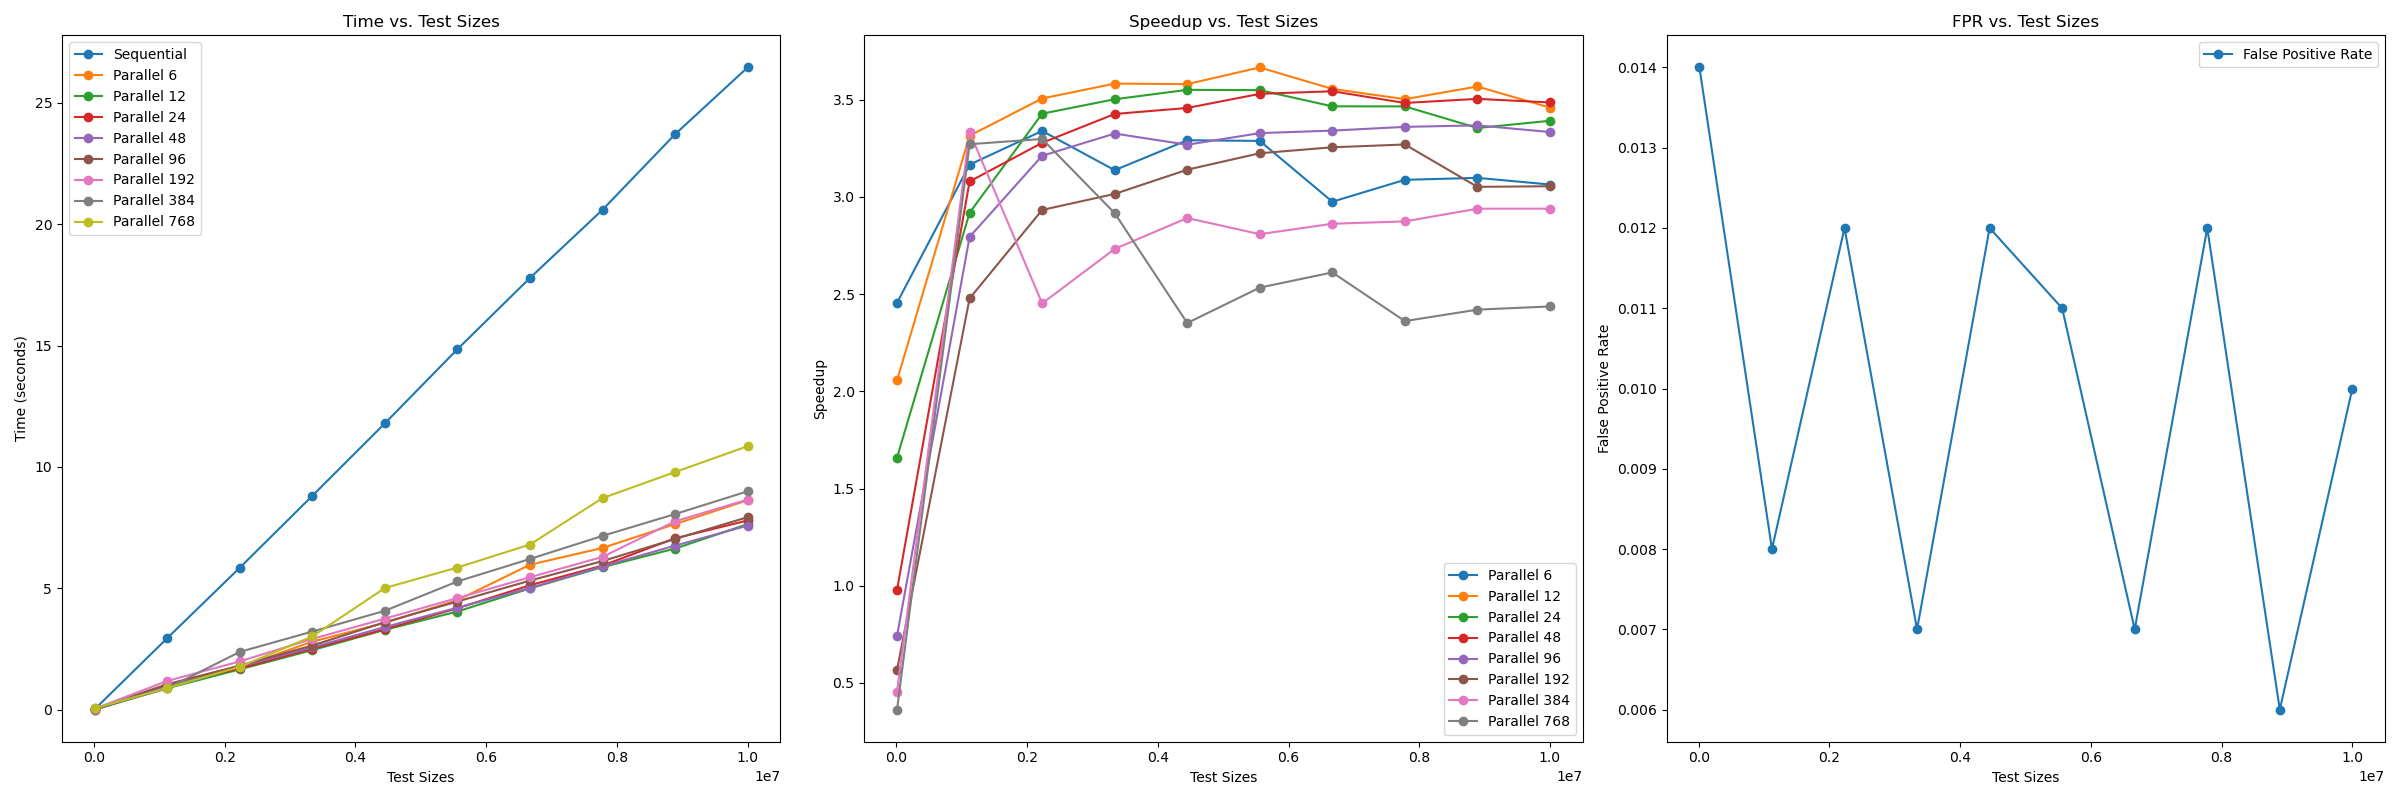
\includegraphics[width=\textwidth]{plot_chunks}
        \caption{Risultati dei test OMP}\label{fig:omp-result}
    \end{figure}

    \section{Conclusioni}\label{sec:conclusioni}
    Dai risultati ottenuti possiamo vedere come il valore di Speedup massimo si attesti intorno a 3 rispetto alla versione sequenziale.
    In generale possiamo notare come lo speedup aumenti con l'aumentare della dimensione dell'insieme, fino ad un certo punto per la versione Joblib.

    \section{Risultati}\label{sec:risultati}
    \begin{table}
        \csvautotabular{../results/csv/setup.csv}
        \csvautotabular{../results/csv/filter.csv}
        \csvautotabular{../results/csv/chunks.csv}
        \caption{Risultati dei test OMP}\label{tab:omp-result-csv}
    \end{table}

    \begin{table}
        \csvautotabular{../results/csv/setup.csv}
        \csvautotabular{../results/csv/filter.csv}
        \csvautotabular{../results/csv/chunks.csv}
        \caption{Risultati dei test Joblib}\label{tab:joblib-result-csv}
    \end{table}

\end{document}